\chapter{Data and MC samples}
\label{chap:data_mc}

\section{Data samples}
\label{sec:data_mc:data}

The analysis uses the 2016 $pp$ collisions data (periods A-L) with the integrated luminosity of 32.8 $\mathrm{fb^{-1}}$. In this search, because the standard ATLAS track reconstruction does not provide good sensitivity for long-lived particles, a dedicated physics stream, \texttt{DRAW\_RPVLL}, is used to reconstruct events using the non-standard reconstruction as described in Chapter~\ref{chap:reco}. The stream is used in several Exotics and SUSY analyses, searching for long-lived particles. %non-standard reconstruction objects.

In this stream, a subset of events from the main physics stream is selected by \texttt{RPVLL} filters. The filters select events using the HLT and offline selections configured for each analysis. The triggers and offline selection used in this search is discussed in Chapter~\ref{chap:signal_selection}. The selected events are passed downstream for reconstruction. The data is in \texttt{RAW} format so that low-level information such as detector hits can be used for the special reconstruction algorithms to reconstruct displaced tracks and vertices.

The events passing HLTs are processed by a sequence of reconstruction algorithms with varying configurations, and the ATLAS metadate interface (AMI) tags are used to specify the configurations to be used for a data processing chain. In this analysis, the events are centrally processed with AMI tag \texttt{r8669} in which the dedicated track reconstruction algorithm, the LRT, and the secondary vertex reconstruction algorithm are enabled to reconstruct tracks and vertices, respectively. The output of \texttt{DRAW\_RPVLL} stream is in \texttt{DAOD\_RPVLL} format which is a standard \texttt{xAOD} data format with additional displaced tracks and secondary vertices reconstructed. 

The \texttt{DAOD\_RPVLL} is further processed to produce the \texttt{DAOD\_SUSY15} derivation for data reduction and software fixes on analysis objects such as energy calibration\footnote{Software fixes are released by the ATLAS collaboration in the form of \texttt{AODfix}.}, as recommended by the Analysis Model Study Group (AMSG)~\cite{Catmore:1543445}. Table~\ref{table:data_samples} summarizes datasets used in this search.

\begin{table}[!htb]
  \centering
  \resizebox{\textwidth}{!}{
    \begin{tabular}{ l l }
      \hline
      \hline
      Format     				& Dataset       													\\
      \hline
      \texttt{DRAW\_RPVLL}	& data16\_13TeV.*.physics\_Main.merge.DRAW\_RPVLL.f*\_m*			\\
      \texttt{DAOD\_RPVLL}	& data16\_13TeV.*.physics\_Main.recon.DAOD\_RPVLL.f*\_r8669			\\
      \texttt{DAOD\_SUSY15}	& data16\_13TeV.*.physics\_Main.recon.DAOD\_RPVLL.f*\_r8669\_p3185	\\
      \hline
      \hline
    \end{tabular}
  }
  \caption{Dataset used in \texttt{DRAW\_RPVLL}, \texttt{DAOD\_RPVLL}, and \texttt{DAOD\_SUSY15} format.}
  \label{table:data_samples}
\end{table}

This search uses a modified version of the standard \texttt{GoodRunsList} because a small number of events selected by \texttt{DRAW\_RPVLL} was not reconstructed successfully. The corresponding luminosity blocks were removed from the \texttt{GoodRunsList}\footnote{\url{data16\_13TeV.periodAllYear\_DetStatus-v83-pro20-15\_DQDefects-00-02-04\_PHYS\_StandardGRL\_All\_Good\\\_25ns\_DAOD\_RPVLL\_r8669.xml}}.


The tag and probe studies of Section~\ref{sec:trigger_efficiency} are performed on the standard xAOD dataset using derivations of the performance groups, given in Table~\ref{table:data_samples:tag_probe}.  

\begin{table}[!htb]
  \centering
  \resizebox{\textwidth}{!}{
    \begin{tabular}{ l l }
      \hline
      \hline
      Format     				& Dataset       													            \\
      \hline
      \texttt{DAOD\_EGAM1}	& data16\_13TeV.*.physics\_Main.PhysCont.DAOD\_EGAM1.grp16\_v01\_p3013    \\
      \texttt{DAOD\_MUON1}	& data16\_13TeV.*.physics\_Main.PhysCont.DAOD\_MUON1.grp16\_v01\_p3043	\\
      \hline
      \hline
    \end{tabular}
  }
  \caption{Datasets used for tag and probe studies.}
  \label{table:data_samples:tag_probe}
\end{table}



\section{MC samples}
\label{sec:mc_sample}

\subsection{Signal samples}
\label{sec:signal_sample}
The long-lived $Z'$ is generated using \texttt{PYTHIA 6.4}~\cite{1126-6708-2006-05-026} with the \texttt{NNPDF23LO} PDF set~\cite{Ball:2014uwa} and the min-bias tune \texttt{A14}. In this signal samples, $Z'$ is singly produced from $q\bar{q}$ scattering and decays to a $\mu\mu$, $ee$, or $e\mu$ pair. The proper lifetime, $c\tau$, is set to 100, 250, or 500 mm. The mass of $Z'$ is set between 100 and 1000 GeV. A width based on relativistic Breit-Wigner is assumed for the new resonance. A sample of 20k events are generated for each mass and lifetime. Table~\ref{table:MC_signal_samples} summarizes dataset identifiers (DIDs), mass, width, and lifetime of the signal MC samples used in this search.

\begin{table}[!htb]
  \centering
  \begin{tabular}{ c c c c c c c }
    \hline
    \hline
           &   &    & \multicolumn{3}{c}{DID}                 \\
    $m_{Z'}$ (GeV) & $\Gamma$ (GeV) & $c\tau$ (mm) &$\mu\mu$ & $ee$ & $e\mu$ \\
    \hline
    100			   &	2.8         &   100	& 308264	& 309539		&	309554		\\
    100			   &	2.8         &   250	& 308265	& 309540		&	309555		\\
    100			   &	2.8         &   500	& 308266	& 309541		&	309556		\\
    250			   &   6.9	        &   100	& 301911	& 309542		&	309557		\\
    250			   &	6.9         &   250	& 301912	& 309543		&	309558		\\
    250			   &	6.9         &   500	& 301913	& 309544		&	309559		\\
    500			   &   14.7         &   100	& 301914	& 309545		&	309560		\\
    500			   &	14.7        &   250	& 301915	& 309546		&	309561		\\
    500			   &	14.7        &   500	& 301916	& 309547		&	309562		\\
    750			   &	23.0        &   100	& 308285	& 309548		&	309563		\\
    750			   &	23.0        &   250	& 308286	& 309549		&	309564		\\
    750			   &	23.0        &   500	& 308287	& 309550		&	309565		\\
    1000	       &	31.0        &   100	& 301917	& 309551		&	309566		\\
    1000	       &	31.0        &   250	& 301918	& 309552		&	309567		\\
    1000	       &	31.0        &   500	& 301919	& 309553		&	309568		\\
    \hline
    \hline
  \end{tabular}
  \caption{Mass, lifetime, and DID of the signal MC samples.}
  \label{table:MC_signal_samples}
\end{table}

The signal MC samples generated using \texttt{PYTHIA} are processed to include detector simulation using the AMI tags \texttt{s2698} and \texttt{s2726}. The samples are overlaid with simulated minimum-bias events to model multiple interactions (pile-up) in data samples. In the signal MC samples, the average number of pile-ups, $\langle\mu\rangle$, ranges from 10 to 40 with small number of events having $\langle\mu\rangle$ < 10. The difference in the $\langle\mu\rangle$ distributions between MC and data samples are corrected for by pile-up reweighting. The resulting MC samples are reconstructed using AMI tag \texttt{r8788}.

In the reconstruction process, the LRT and the secondary vertex reconstruction algorithms are used with the same configuration as data samples to reconstruct displaced tracks and vertices. The reconstructed events are stored in \texttt{DAOD\_RPVLL}, and the samples are processed to produce the \texttt{DAOD\_SUSY15} derivation for data reduction and software fixes on analysis objects.

The representative plots of generator-level $p_{T}$ and $\eta$ distributions of $Z'$ and the muons from the decay of $Z'$, referred as \textit{signal} muons, are shown in Figure~\ref{fig:truth_zp_muon} using the signal MC samples with $m=$ 500, 1000 GeV and $c\tau=$ 100 mm. %The signal MC samples with $ee$ and $e\mu$ final states produce similar distributions as shown in Appendix~\ref{app:signal_truth}.

%The $\eta$ distribution of $Z'$ shows a forward distribution, and it is reweighted to a flat $\eta$ distribution to provide model-independent result. The details are discussed in Section~\ref{sec:efficiency_reweighting}.
The $\eta$ distribution of signal muons shows that most of the signal muons are produced within the detector acceptance ($\eta <$ 2.7). The characteristic upper edge in the $p_{T}$ spectrum is related to the $Z'$ mass.
%The $p_{T}$ distribution of muons shows that muon $p_{T}$ is constrained by the $Z'$ mass.


\begin{figure}[!htb]
    \centering
    \subfloat[]{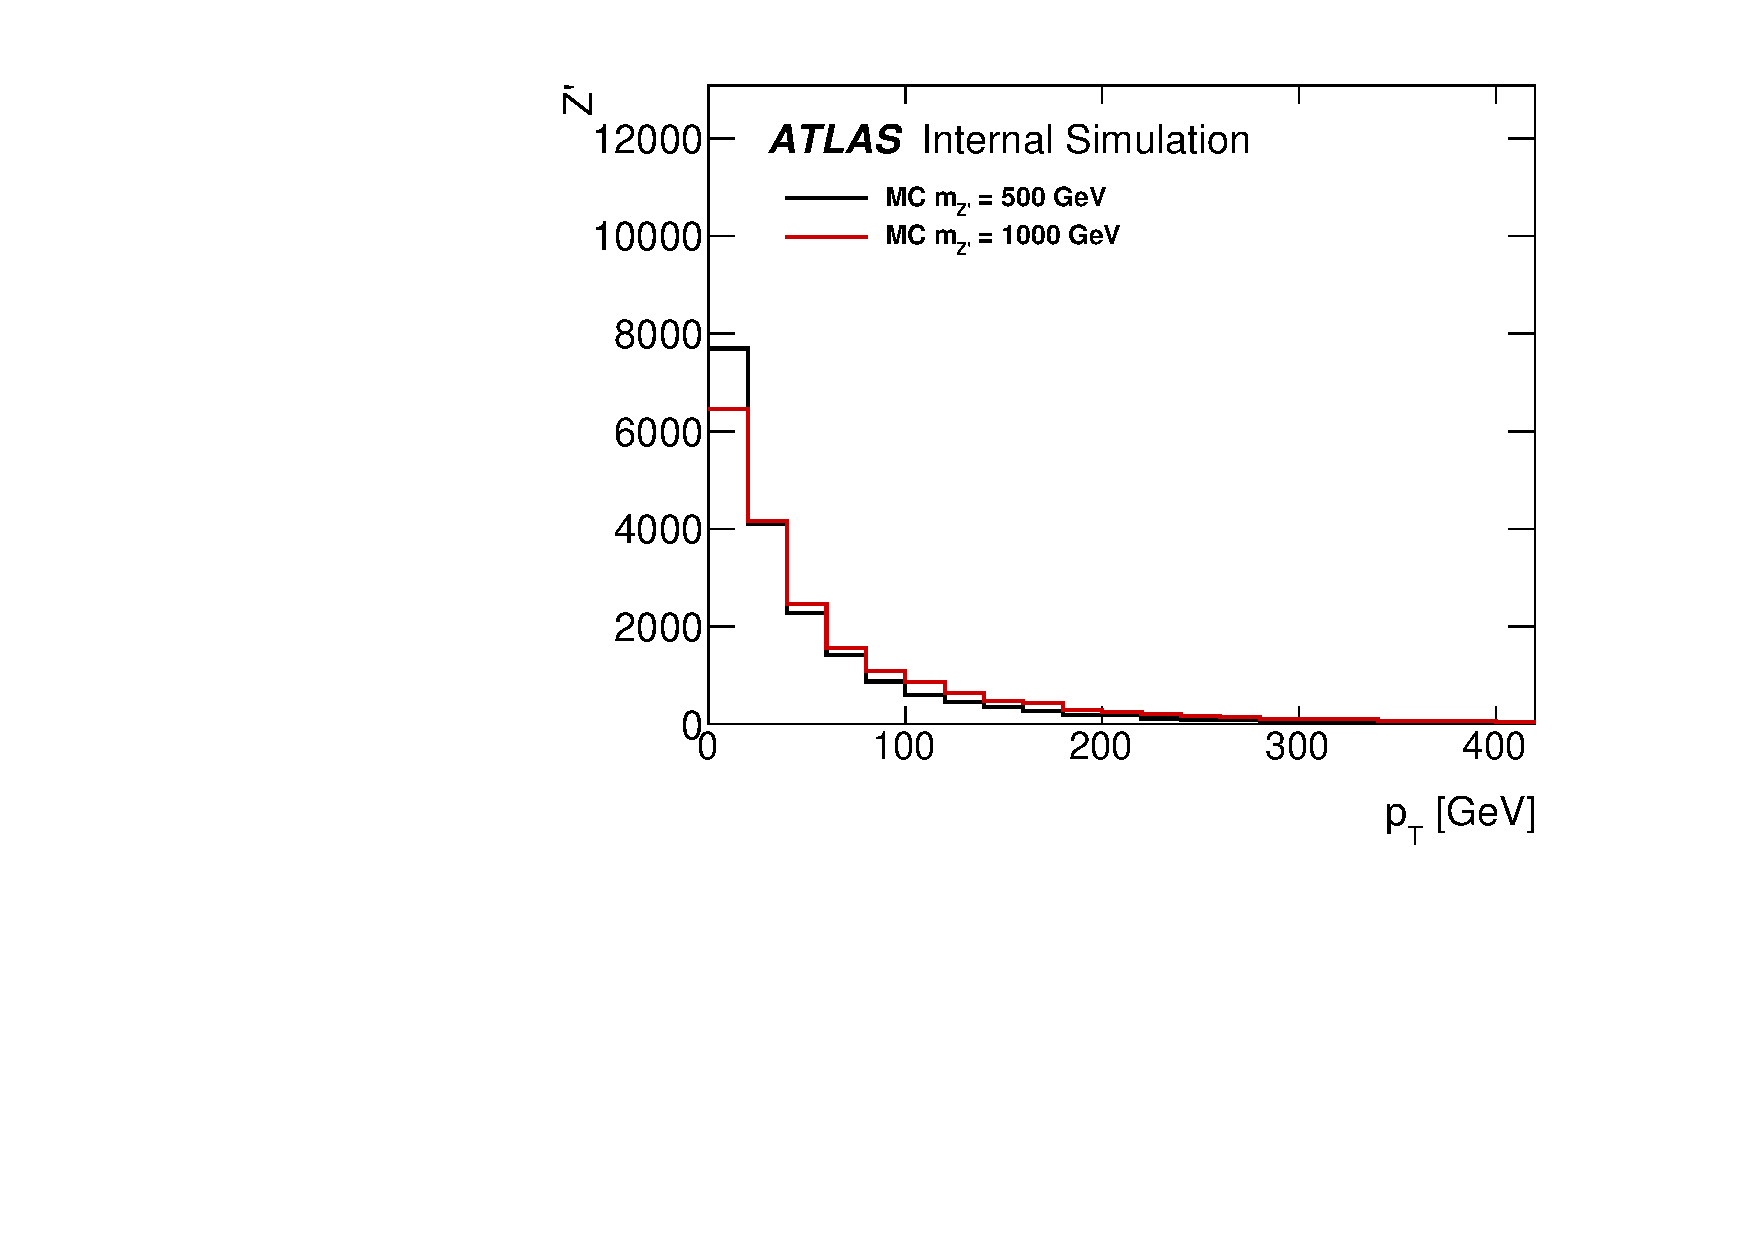
\includegraphics[width=0.45\textwidth]{figures/m_truth_zp_pt.pdf}}
    \subfloat[]{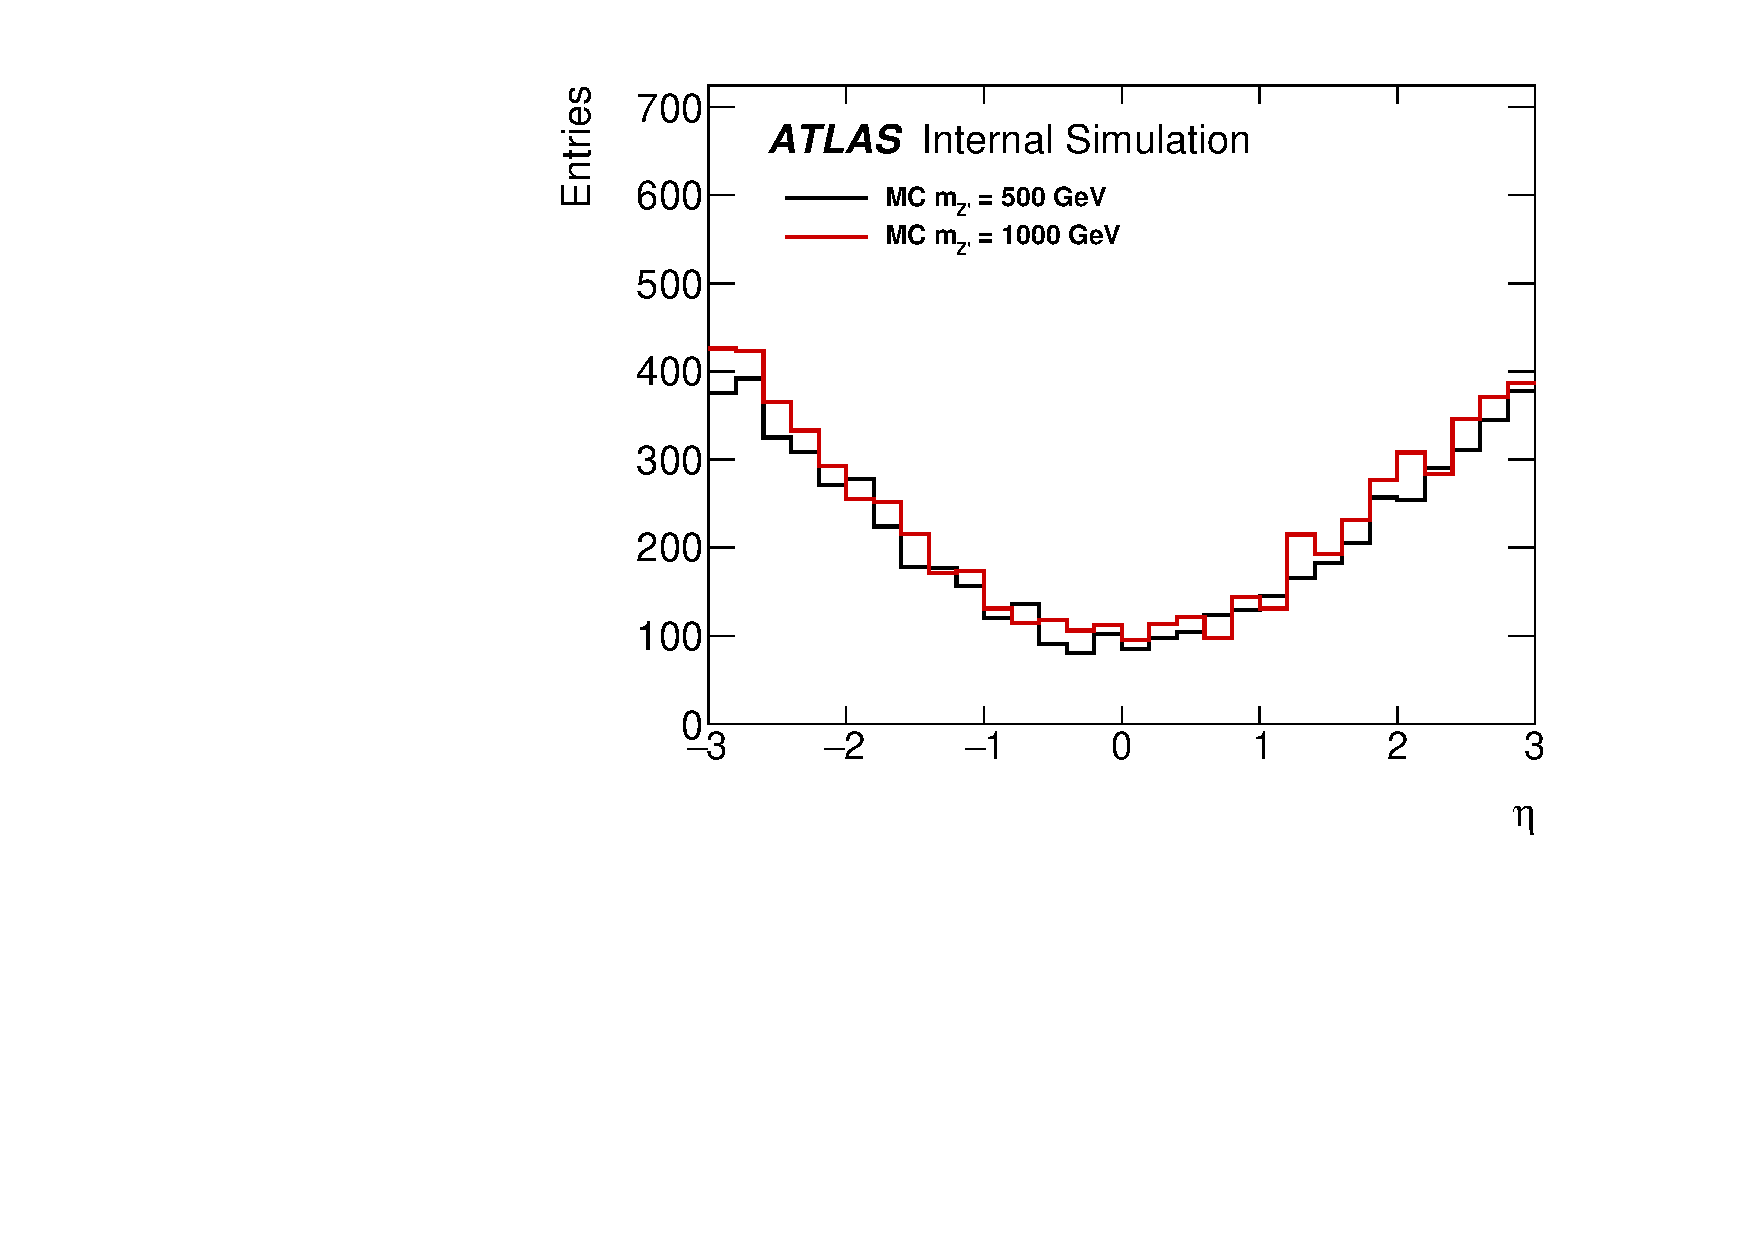
\includegraphics[width=0.45\textwidth]{figures/m_truth_zp_eta.pdf}} \\
    \subfloat[]{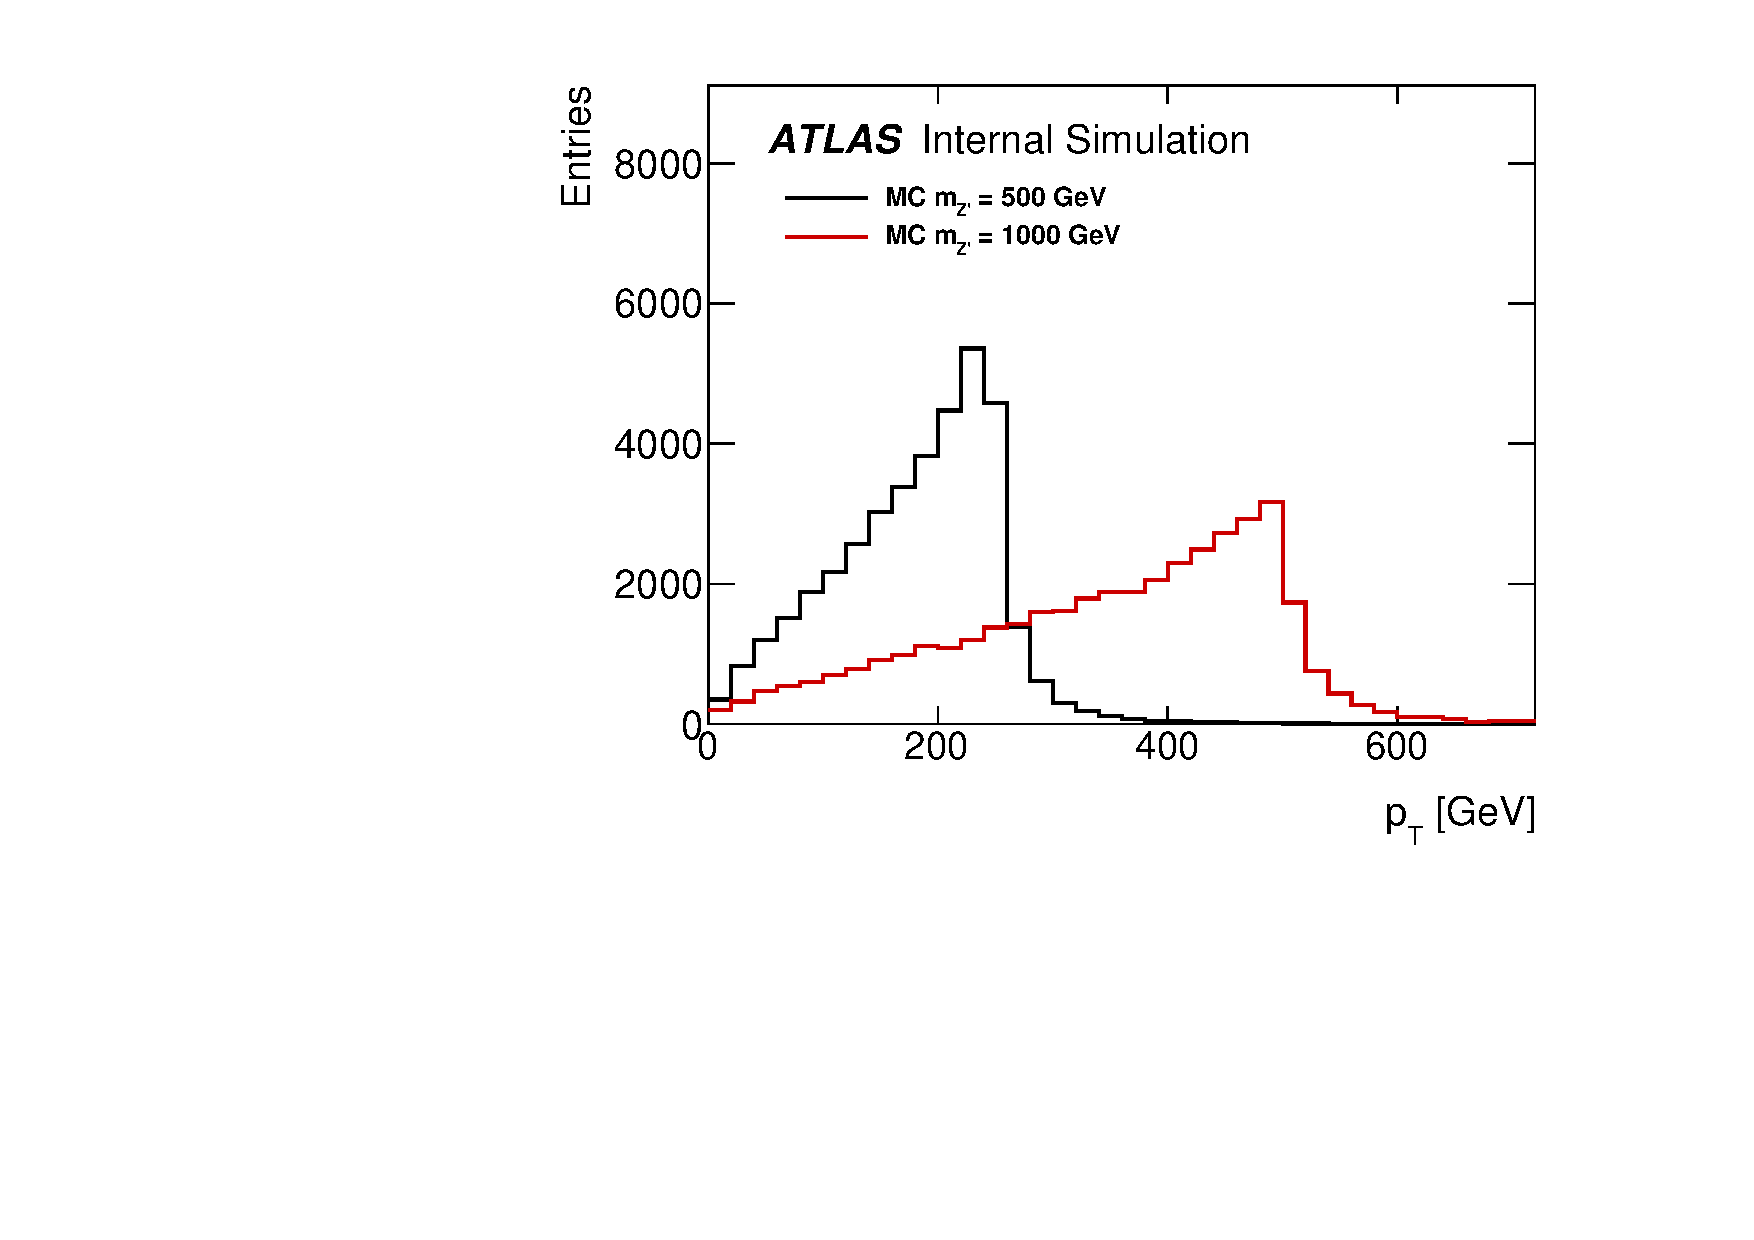
\includegraphics[width=0.45\textwidth]{figures/m_truth_muon_pt.pdf}}
    \subfloat[]{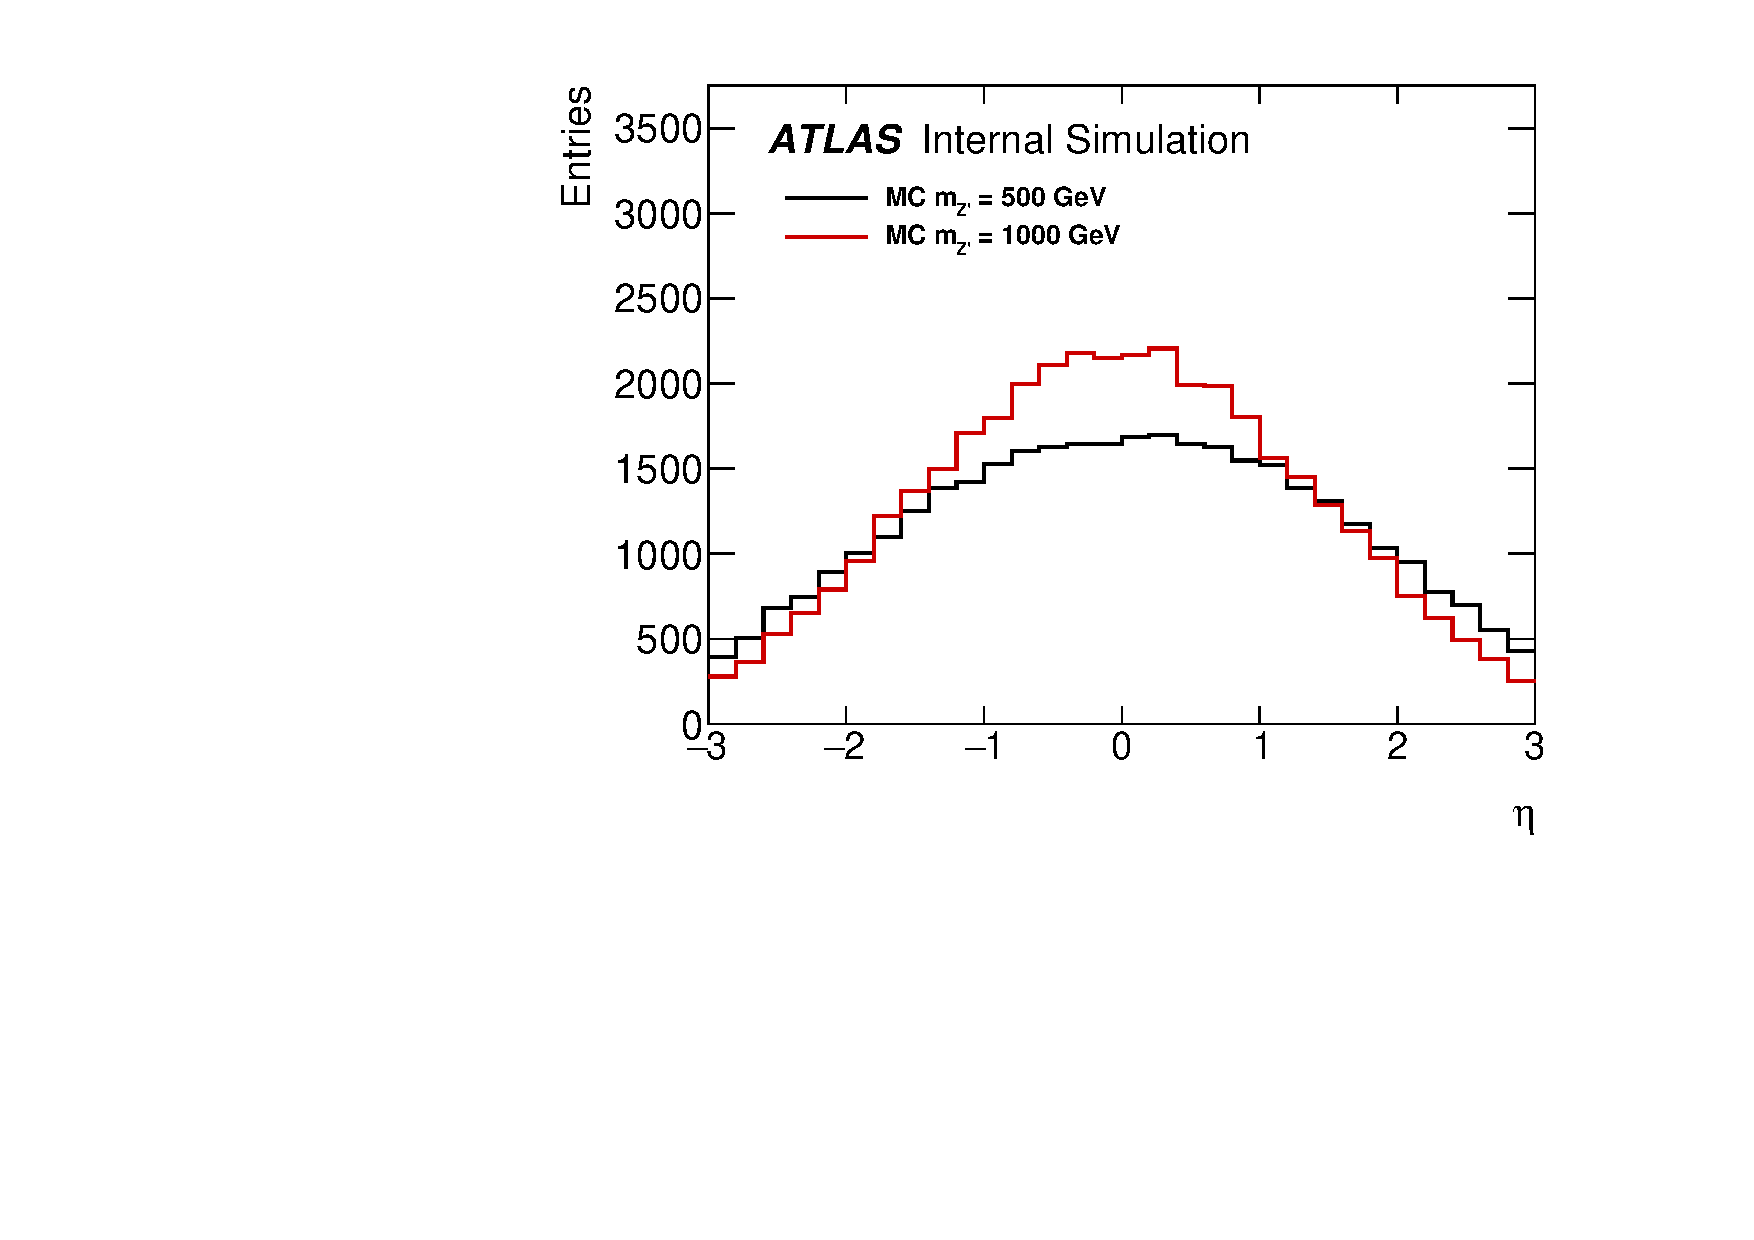
\includegraphics[width=0.45\textwidth]{figures/m_truth_muon_eta.pdf}}
    \caption{The representative plots of generator-level (a) $p_{T}$ and (b) $\eta$ distributions of $Z'$, and (c), (d) are the corresponding distributions for the signal muons. The signal MC samples are generated with $m=$ 500, 1000 GeV, and $c\tau=$ 100 mm.}
    \label{fig:truth_zp_muon}
\end{figure}


\subsection{Background MC samples}
\label{sec:background_mc_sample}
In this analysis, backgrounds are estimated from data because most of the backgrounds are expected to be originated from non-collision processes such as cosmic rays or random-crossing of tracks. %sources other than the SM collision process 

However, SM background samples are used to study the performance of random-crossing background estimation (Section~\ref{sec:bkg:random}) and to estimate the systematic uncertainties in vertexing and tracking (Section~\ref{sec:syst:vertexing}). The $t\bar{t}$ samples are generated for QCD background study using \texttt{SHERPA}~\cite{Gleisberg:2008ta} with the \texttt{NNPDF30NNLO} PDF set. The samples with leptonic decay of di-boson ($ZZ$, $WW$, $W^{\pm}Z$) are generated using \texttt{SHERPA} with the \texttt{CT10} PDF set. The di-jet samples (JZ3W-JZ7W) are generated in slices of leading jet $p_{T}$ (160-400, 400-800, 800-1300, 1300-1800, 1800-2500 GeV) using \texttt{PYTHIA8} with \texttt{NNPDF23LO} PDF set. These samples are sufficient for testing purposes, as they contain high-$p_{T}$ isolated leptons (from $W$ boson decays) and leptons and displaced tracks in $b$-jets, in addition to tracks from pile-up vertices. Details on the PDF sets can be found in Ref.~\cite{Ball:2014uwa}.

The SM background samples are reprocessed using the same configuration as the signal MC sample for consistency. The background MC samples used for background and systematic uncertainty estimations are summarized in Table~\ref{table:background_MC}.


\begin{table}[!htb]
  \centering
  \begin{tabular}{ l l l l l}
    \hline
    \hline
    Process         &   DID     &   $\sigma$ (pb)       & Events ($10^{6}$) &   $\mathcal{L}_{Int} (\mathrm{fb^{-1}})$ \\
    \hline
    $t\bar{t}$                              &   410252  &   87.8   &   0.70        &   7.97                 \\
    $ZZ\rightarrow \ell \ell \ell \ell$     &   361063  &   11.7   &   0.12        &   10.3                 \\
    $W^{-}Z\rightarrow \ell \ell \ell v$    &   361064  &   1.68   &   0.020       &   10.2                 \\
    $W^{+}Z\rightarrow \ell \ell \ell v$    &   361066  &   2.33   &   0.025       &   30.0                 \\
    $WW \rightarrow \ell \ell vv$           &   361068  &   12.8   &   0.13        &   1.95                 \\
    JZ3W                                    &   361023  &   8.45$\cdot10^{3}$      &   0.20  &   0.0247     \\
    JZ4W                                    &   361024  &   135    &   0.20        &   1.48                 \\
    JZ5W                                    &   361025  &   4.20   &   0.20        &   47.6                 \\
    JZ6W                                    &   361026  &   2.42$\cdot10^{-2}$     &   0.20  &   826        \\
    %$t\bar{t}$                              &   410252  &   76.3   &   0.70        &   9.17                 \\
    %$ZZ\rightarrow \ell \ell \ell \ell$     &   361063  &   12.8   &   0.12        &   9.30                 \\
    %$W^{-}Z\rightarrow \ell \ell \ell v$    &   361064  &   1.84   &   0.020       &   10.9                 \\
    %$W^{+}Z\rightarrow \ell \ell \ell v$    &   361066  &   2.56   &   0.025       &   9.77                 \\
    %$WW \rightarrow \ell \ell vv$           &   361068  &   14.0   &   0.13        &   9.29                 \\
    %JZ3W                                    &   361023  &   2.65$\cdot10^{7}$      &   0.20  &   < $10^{-5}$\\
    %JZ4W                                    &   361024  &   0.255  &   0.20        &   784                  \\
    %JZ5W                                    &   361025  &   0.455  &   0.20        &   440                  \\
    %JZ6W                                    &   361026  &   258    &   0.20  &   0.775      \\
    %JZ7W                                    &   361027  &   16.2                   &   0.10  &   0.617      \\
    \hline
    \hline
  \end{tabular}
  \caption{Background MC samples used in the study of random-crossing background and in the estimation of tracking and vertexing systematic uncertainty.}
  \label{table:background_MC}
\end{table}


Additional samples are used without the special reconstruction to study the efficiency of the triggers using tag-and-probe method (Section~\ref{sec:trigger_efficiency}). These samples are given in Table~\ref{table:background_MC:tag_probe}.

%\begin{table}[!htb]
\begin{sidewaystable}[!htb]
  \centering
  \resizebox{\textwidth}{!}{
    \begin{tabular}{ l l }
      \hline
      \hline
      Format     				& Dataset       													            \\
      \hline
      \texttt{DAOD\_EGAM1}	& mc15\_13TeV.361106.PowhegPythia8EvtGen\_AZNLOCTEQ6L1\_Zee.merge.DAOD\_EGAM1.e3601\_s2576\_s2132\_r7725\_r7676\_p3012  \\
      \texttt{DAOD\_MUON1}	& mc15\_13TeV.361107.PowhegPythia8EvtGen\_AZNLOCTEQ6L1\_Zmumu.merge.DAOD\_MUON1.e3601\_s2576\_s2132\_r7725\_r7676\_p3045	\\
      \hline
      \hline
    \end{tabular}
  }
  \caption{Background MC samples without the LRT used for tag and probe studies.}
  \label{table:background_MC:tag_probe}
%\end{table}
\end{sidewaystable}




